\documentclass[border=10pt, multi, tikz]{standalone}
\usetikzlibrary{positioning,fit,arrows.meta,backgrounds}
\usepackage{amsmath,amssymb}

\definecolor{simcol}{RGB}{214,239,216}
\definecolor{datacol}{RGB}{255,243,205}
\definecolor{netcol}{RGB}{222,226,255}
\definecolor{headcol}{RGB}{240,224,255}
\definecolor{mcmccol}{RGB}{224,247,250}
\definecolor{valcol}{RGB}{255,224,230}
\definecolor{band}{RGB}{245,245,245}

\begin{document}
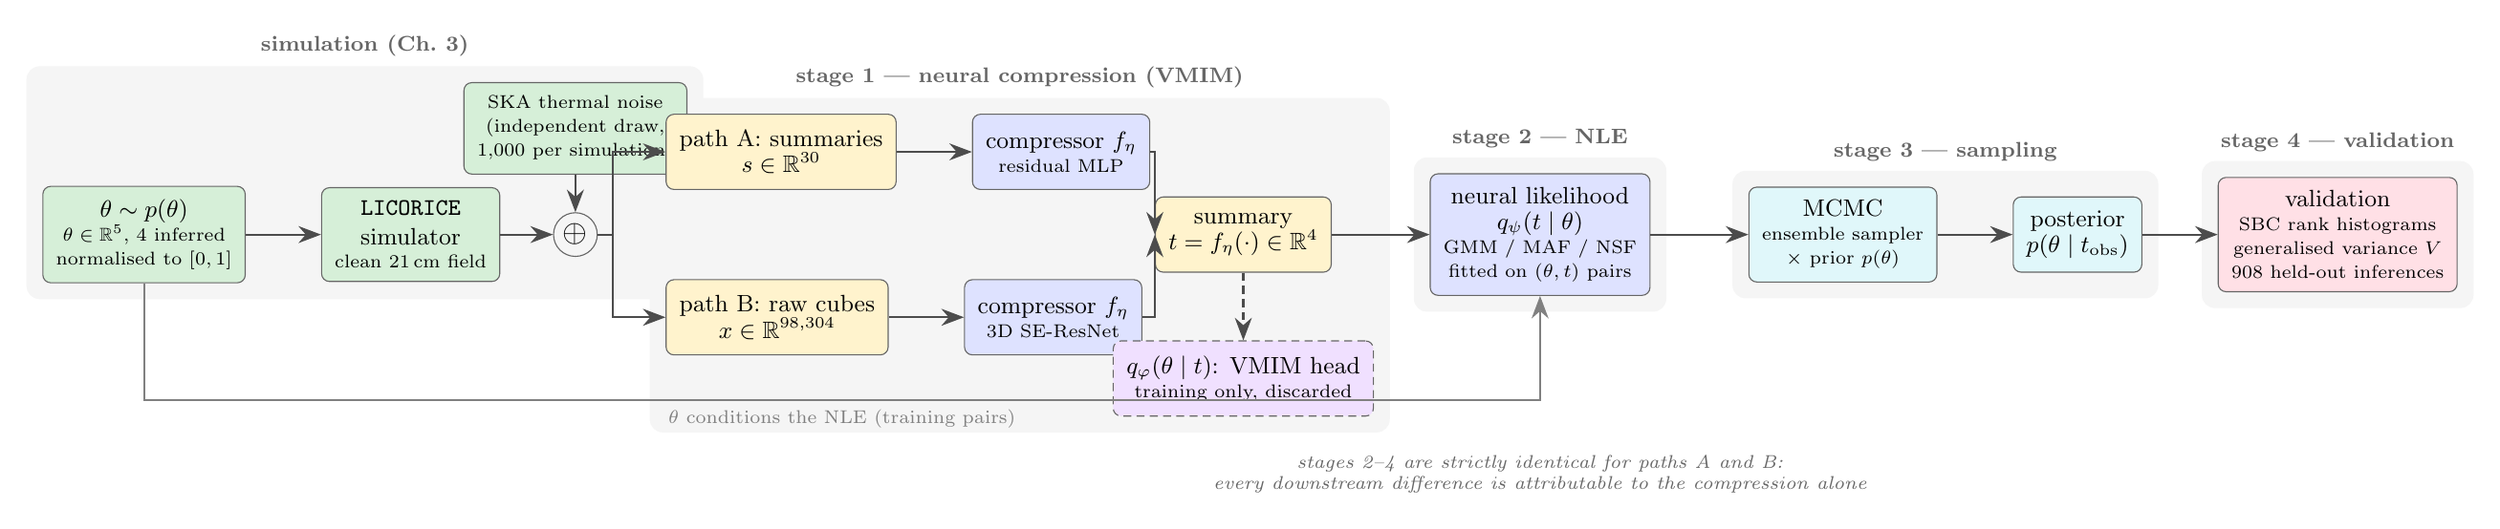
\begin{tikzpicture}[
  node distance=7mm and 10mm,
  every node/.style={font=\small},
  box/.style={draw=black!60, rounded corners=3pt, align=center, inner sep=5pt, minimum height=10mm},
  arr/.style={-{Stealth[length=3mm]}, thick, black!70},
  darr/.style={arr, densely dashed},
  stage/.style={font=\footnotesize\bfseries, text=black!60}
]

% =================== simulation ===================
\node[box, fill=simcol] (theta) {$\theta \sim p(\theta)$\\[-2pt]\scriptsize $\theta\in\mathbb{R}^5$, 4 inferred\\[-2pt]\scriptsize normalised to $[0,1]$};
\node[box, fill=simcol, right=of theta] (sim) {\texttt{LICORICE}\\ simulator\\[-2pt]\scriptsize clean 21\,cm field};
\node[circle, draw=black!60, inner sep=1.5pt, right=7mm of sim, font=\large] (plus) {$\oplus$};
\node[box, fill=simcol, above=5mm of plus, align=center] (noise) {\scriptsize SKA thermal noise\\[-2pt]\scriptsize (independent draw,\\[-2pt]\scriptsize 1{,}000 per simulation)};

% =================== two data representations ===================
\node[box, fill=datacol, right=9mm of plus, yshift=11mm] (s) {path A: summaries\\[-1pt]$s\in\mathbb{R}^{30}$};
\node[box, fill=datacol, right=9mm of plus, yshift=-11mm] (x) {path B: raw cubes\\[-1pt]$x\in\mathbb{R}^{98{,}304}$};

% =================== stage 1: compression ===================
\node[box, fill=netcol, right=of s] (fA) {compressor $f_\eta$\\[-2pt]\scriptsize residual MLP};
\node[box, fill=netcol, right=of x] (fB) {compressor $f_\eta$\\[-2pt]\scriptsize 3D SE-ResNet};
\node[box, fill=datacol, right=30mm of plus, xshift=44mm] (t) {summary\\[-1pt]$t = f_\eta(\cdot)\in\mathbb{R}^{4}$};
\node[box, fill=headcol, densely dashed, below=9mm of t] (head)
  {$q_\varphi(\theta\mid t)$: VMIM head\\[-2pt]\scriptsize training only, discarded};

% =================== stage 2: NLE ===================
\node[box, fill=netcol, right=13mm of t] (nle)
  {neural likelihood\\[-1pt]$q_\psi(t\mid\theta)$\\[-2pt]\scriptsize GMM / MAF / NSF\\[-2pt]\scriptsize fitted on $(\theta,t)$ pairs};

% =================== stage 3: MCMC ===================
\node[box, fill=mcmccol, right=13mm of nle] (mcmc)
  {MCMC\\[-2pt]\scriptsize ensemble sampler\\[-2pt]\scriptsize $\times$ prior $p(\theta)$};
\node[box, fill=mcmccol, right=of mcmc] (post) {posterior\\[-1pt]$p(\theta\mid t_{\mathrm{obs}})$};

% =================== stage 4: validation ===================
\node[box, fill=valcol, right=of post] (val)
  {validation\\[-2pt]\scriptsize SBC rank histograms\\[-2pt]\scriptsize generalised variance $V$\\[-2pt]\scriptsize 908 held-out inferences};

% =================== arrows ===================
\draw[arr] (theta) -- (sim);
\draw[arr] (sim) -- (plus);
\draw[arr] (noise) -- (plus);
\draw[arr] (plus.east) -- ++(2mm,0) |- (s.west);
\draw[arr] (plus.east) -- ++(2mm,0) |- (x.west);
\draw[arr] (s) -- (fA);
\draw[arr] (x) -- (fB);
\draw[arr] (fA.east) -- (t.west|-fA.east) -- (t.west);
\draw[arr] (fB.east) -- (t.west|-fB.east) -- (t.west);
\draw[darr] (t) -- (head);
\draw[arr] (t) -- (nle);
\draw[arr] (nle) -- (mcmc);
\draw[arr] (mcmc) -- (post);
\draw[arr] (post) -- (val);
% theta feeds NLE training (conditioner)
\draw[arr, black!50] (theta.south) -- ++(0,-1.55) -| node[below, font=\scriptsize, pos=0.25]{$\theta$ conditions the NLE (training pairs)} (nle.south);

% =================== stage bands (background) ===================
\begin{scope}[on background layer]
  \node[fill=band, rounded corners=5pt, fit=(theta)(sim)(noise)(plus), inner sep=6pt,
        label={[stage]above:{simulation (Ch.~3)}}] {};
  \node[fill=band, rounded corners=5pt, fit=(s)(x)(fA)(fB)(t)(head), inner sep=6pt,
        label={[stage]above:{stage 1 --- neural compression (VMIM)}}] {};
  \node[fill=band, rounded corners=5pt, fit=(nle), inner sep=6pt,
        label={[stage]above:{stage 2 --- NLE}}] {};
  \node[fill=band, rounded corners=5pt, fit=(mcmc)(post), inner sep=6pt,
        label={[stage]above:{stage 3 --- sampling}}] {};
  \node[fill=band, rounded corners=5pt, fit=(val), inner sep=6pt,
        label={[stage]above:{stage 4 --- validation}}] {};
\end{scope}

% note: identical downstream
\node[align=center, font=\scriptsize\itshape, text=black!60, below=20mm of nle]
  {stages 2--4 are strictly identical for paths A and B:\\ every downstream difference is attributable to the compression alone};

\end{tikzpicture}
\end{document}
